% !TEX root = ../main.tex
\newpage
\chapter{РЕАЛІЗАЦІЯ ПРОГРАМНОЇ ВЗАЄМОДІЇ З БД}
\section{Посібник користувача}
Попередньо на ПК має бути встановлено сервер MySQL 8.0 та інтерпретатор мови програмування Python 3.9.
Після запуску SQL-сервера перед першим запуском інформаційної системи необхідно
запустити файл setup.py (додаток Б, ст. \pageref{setup}), який виконає створення 
схеми БД на сервері, створить усі необхідні таблиці, створить усі необхідні для запитів процедури
та завантажить тестові дані до таблиць:
\begin{lstlisting}[style=code]
PS C:\Users\Yalikesi\...\campus> python setup.py
enter connection parameters:
        host (leave empty for default localhost):
        port (leave empty for default 3307):
        user (leave empty for default root):
        password for root:
creating schema and tables...
        done in 0.997 sec
inserting data...
        done in 0.766 sec
creating stored procedures...
        done in 0.219 sec
database is ready!
\end{lstlisting}
Після цього параметри підключення до БД буде збережено і можна буде запускати веб-інтерфейс за
допомогою файлу main.py: буде виведено рядок \inlinecode{Running on http://127.0.0.1:5000/ (Press CTRL+C to quit)},
який означатиме, що веб-інтерфейс доступний за адресою 127.0.0.1:5000. Його можна відкрити за допомогою
будь-якого сучасного браузера. Під час тестування коректність його роботи перевірялася в Google Chrome 90.
У веб-інтерфейсі є можливість перегляду окремих таблиць БД та виконання передбачених запитів.
На всіх сторінках, де виводяться таблиці, є можливість сортування за кожним стовпцем та пошуку по виведеній таблиці.
Усі необхідні параметри запитів користувач обирає за допомогою HTML-форм, які мають обмежені задані варіанти значень, що
унеможливлює передачу некоректних параметрів запиту. Єдиною виключною ситуацію є введення такої комбінації параметрів,
яка гарантовано дасть порожній результат запиту: наприклад, якщо обрати одночасно факультет та групу, яка до нього не належить. 
\begin{figure}[H]
    \centering
    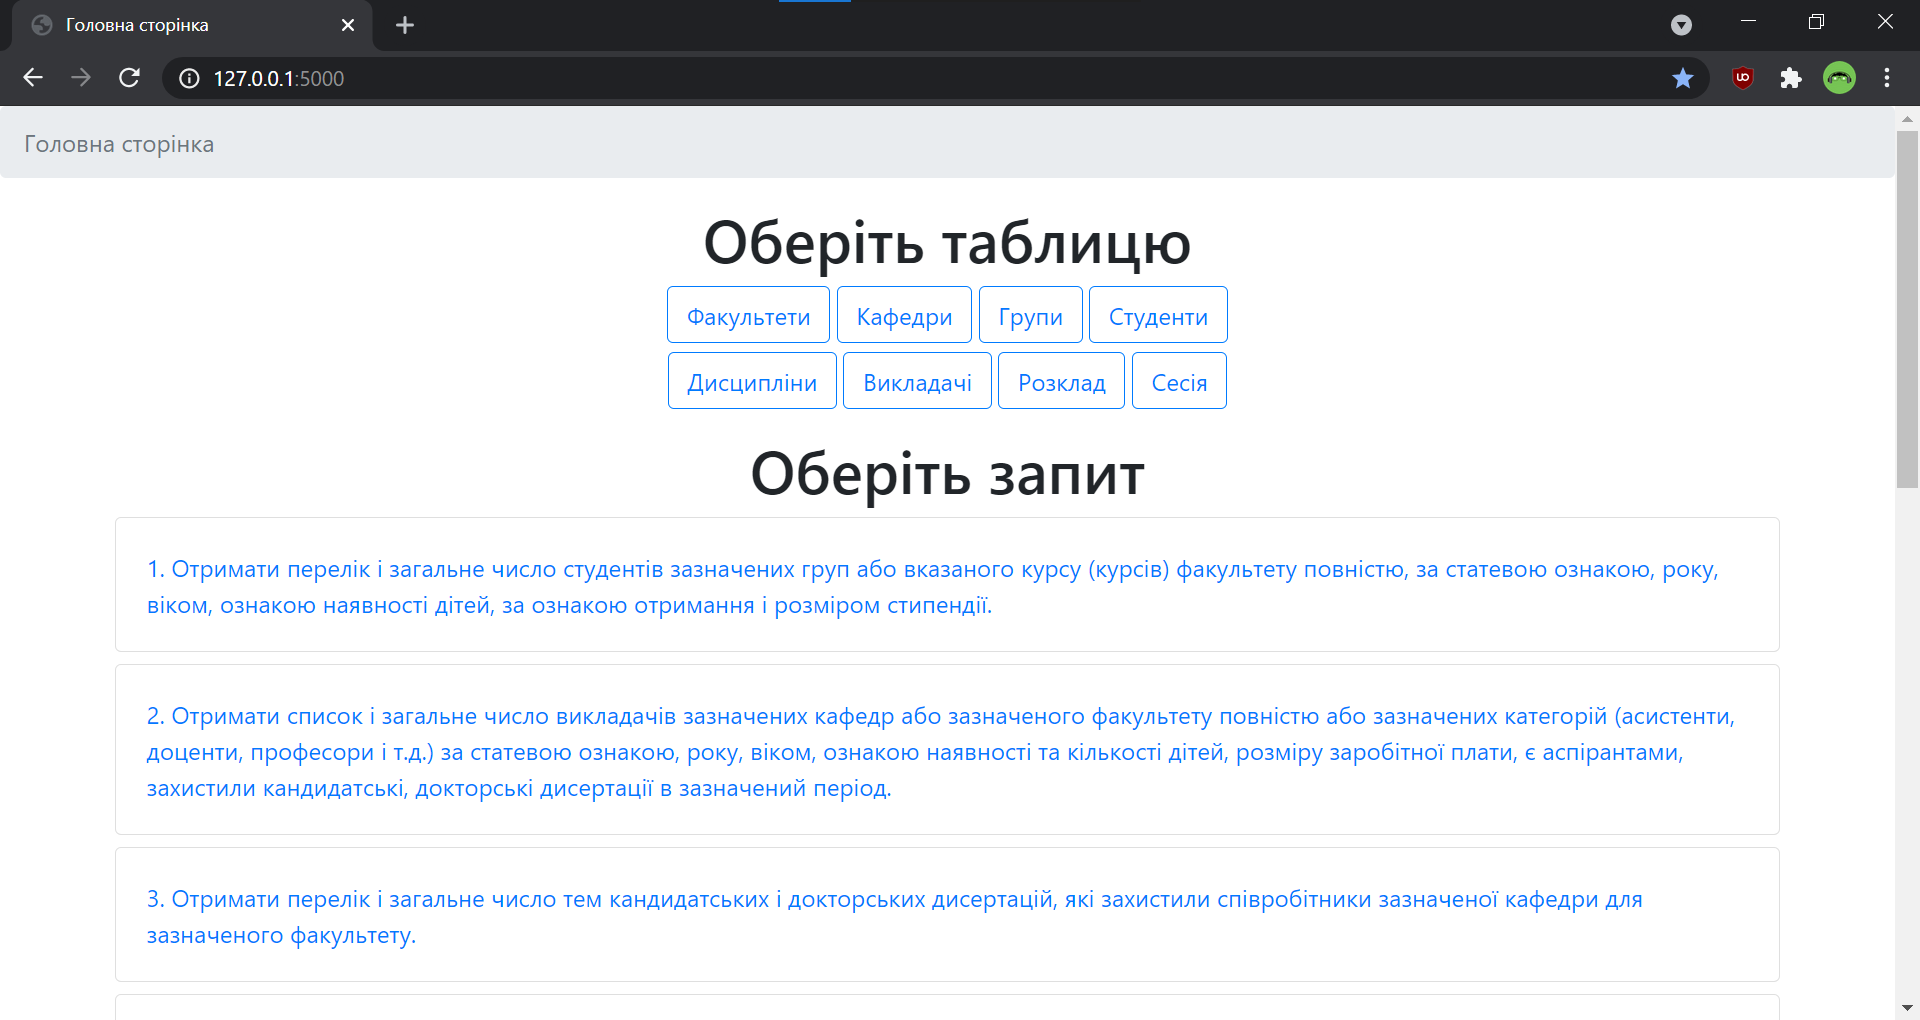
\includegraphics[scale=0.38]{pics/web_main.png}
    \caption{Головна сторінка веб-інтерфейсу}
\end{figure}

\begin{figure}[H]
    \centering
    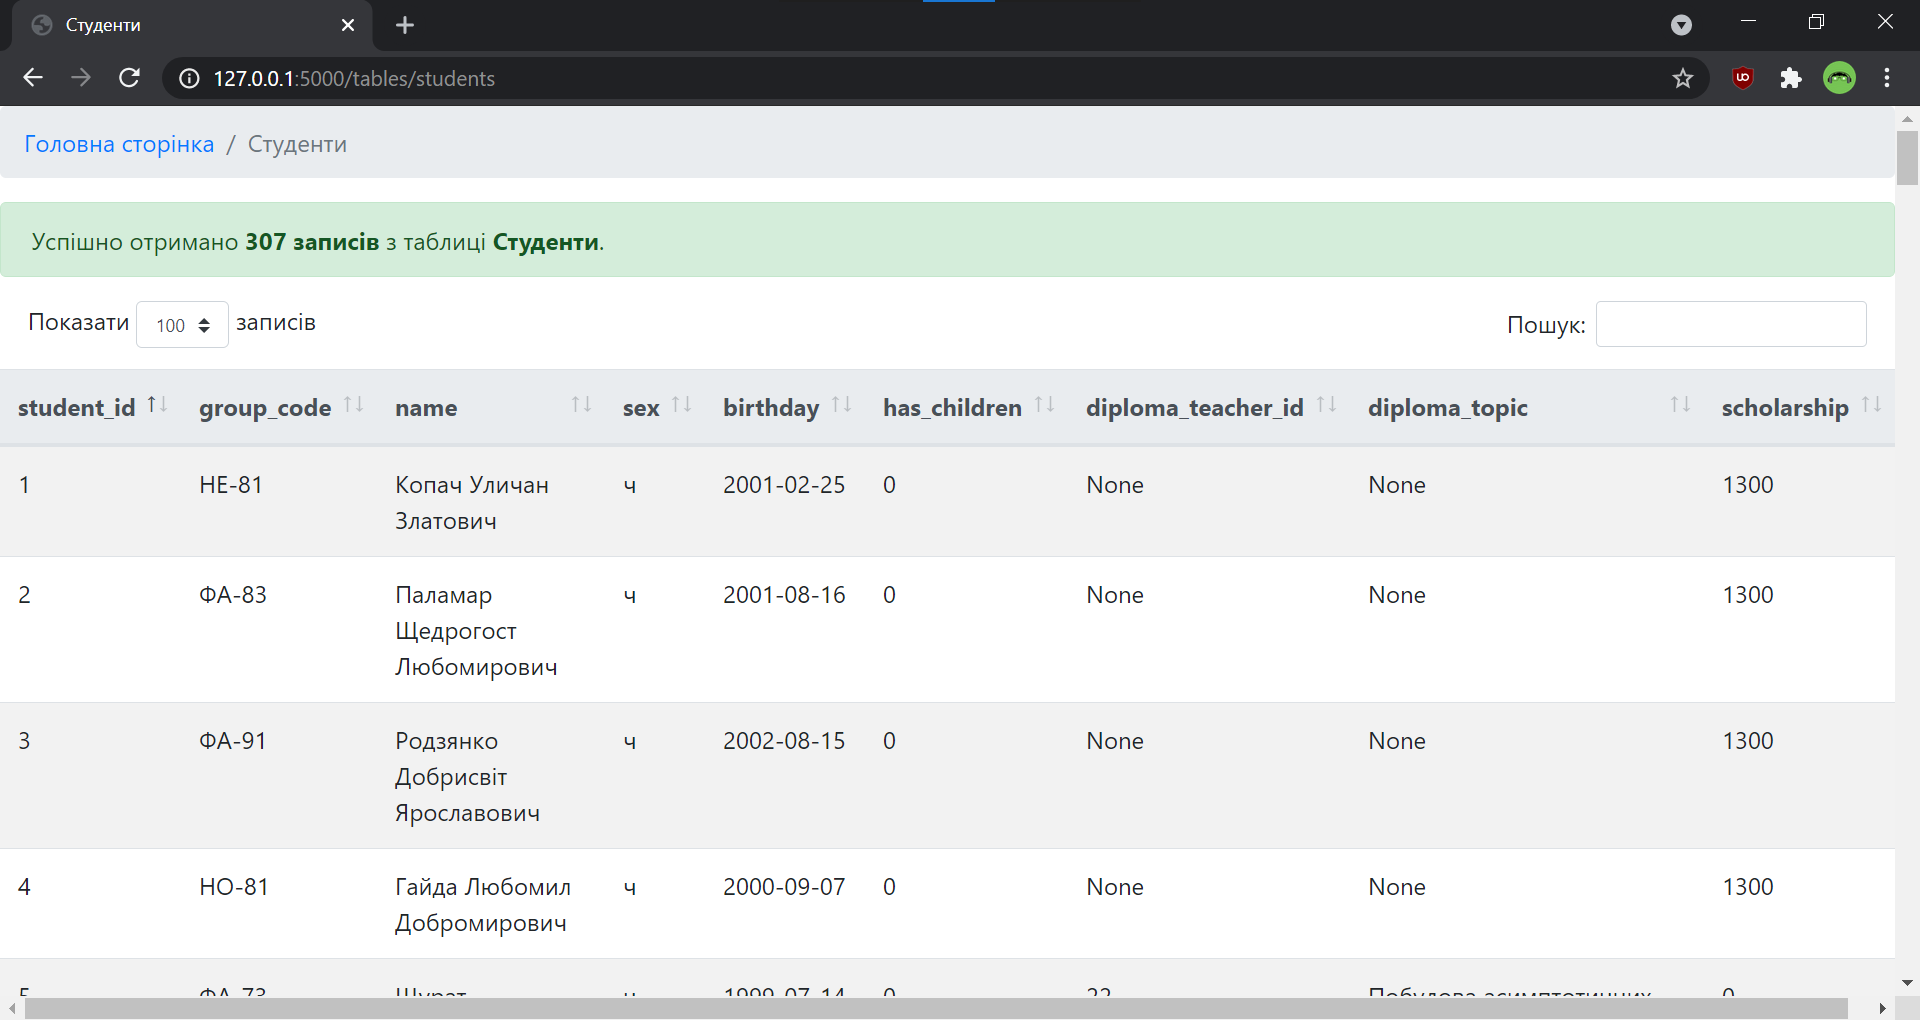
\includegraphics[scale=0.38]{pics/web_table.png}
    \caption{Перегляд таблиці <<Студенти>>}
\end{figure}

\begin{figure}[H]
    \centering
    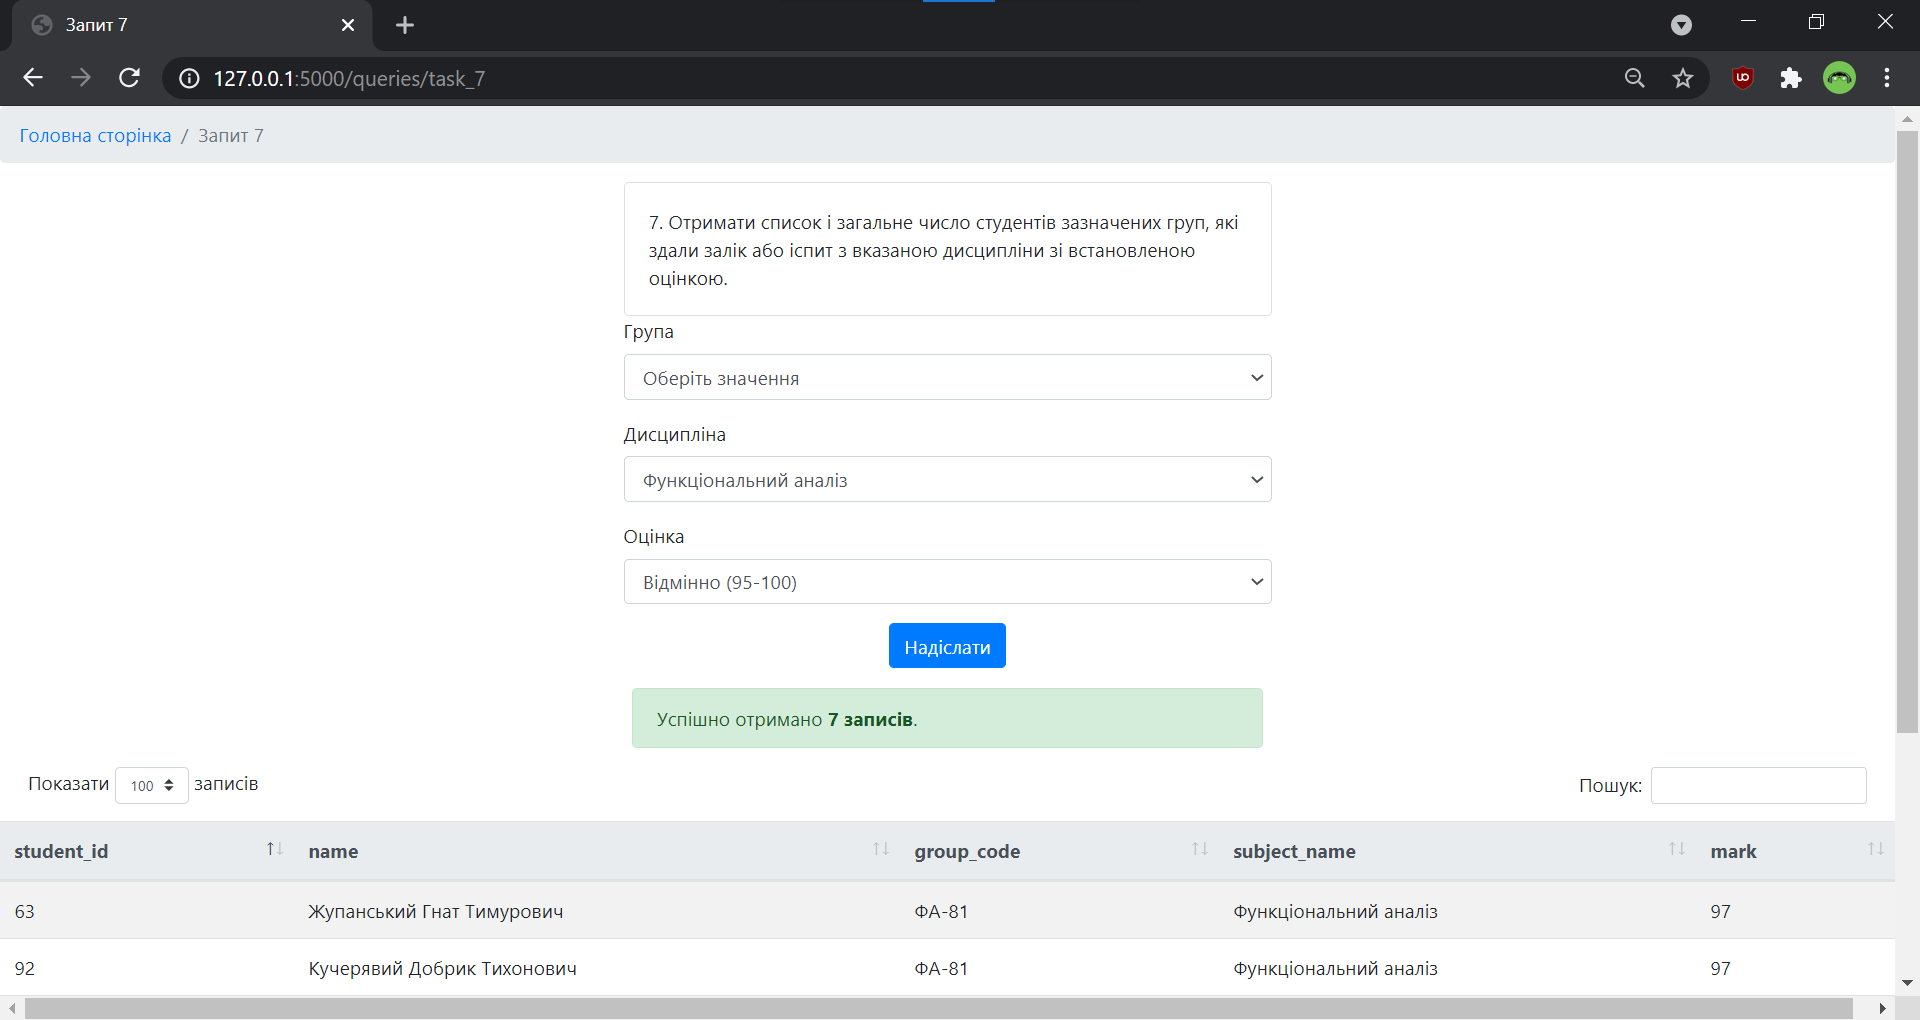
\includegraphics[scale=0.38]{pics/web_query.png}
    \caption{Форма для запиту та результат виконання}
\end{figure}

\section{Реалізація механізмів БД}
Реалізовано 13 процедур, що відповідають поставленим вимогам до запитів.
SQL-код цих процедур наведено в додатку В, ст. \pageref{queries}. Виклик усіх процедур
відбувається через веб-інтерфейс і користувачу не потрібно писати назву чи параметри процедури вручну.
У всіх процедурах реалізовано можливість передавати параметри у будь-якій їх комбінації: якщо у веб-інтерфейсі
значення деякого параметру не вказано, то замість нього передається значення -1, а в самому запиті спочатку робиться вибірка з потрібної
таблиці без врахування параметрів, а потім по черзі перевіряються значення параметрів і, якщо деякий параметр вказано, то з вибірки
прибираються значення, які йому не відповідають.
На прикладі запиту <<отримати список студентів і тем дипломних робіт на зазначеній кафедрі або у зазначеного викладача>>:
параметрами цього запиту є \inlinecode{chair\_id} та \inlinecode{teacher\_id}. Спочатку з таблиці <<Студенти>> робиться вибірка
всіх студентів з дипломними керівниками:
\begin{lstlisting}[language=SQL, style=code]
drop table if exists temp_table;
create table temp_table select * from `students` where diploma_teacher_id is not NULL;
\end{lstlisting}
Після цього по черзі перевіряється, чи задано параметри запиту:
\begin{lstlisting}[language=SQL, style=code]
if `teacher_id` != -1 then
	delete from temp_table where temp_table.diploma_teacher_id != `teacher_id`;
end if;
if `chair_id` != -1 then
	delete t1 from temp_table t1 join `teachers` t2 on t1.diploma_teacher_id = t2.teacher_id
        and t2.chair_id != `chair_id`;
end if;
\end{lstlisting}
Тобто, якщо вказано викладача, то з вибірки прибираються всі студенти, у яких дипломний керівник інший, так само і з вказанням
кафедри.
\section{Вимоги до апаратних і програмних засобів}
Для роботи з інформаційною системою необхідно мати ПК з встановленим MySQL Server 8.0, інтерпретатором мови програмування Python 3.9 з
встановленими найновішими версіями фреймворку Flask і бібліотек PyMySQL та cryptography, які встановлюються за допомогою
системи керування пакетами Python pip командами \inlinecode{pip install -U Flask PyMySQL cryptography}.

\section{Випробування розроблених програм}
Було перевірено роботу усіх 13 запитів, які необхідно було реалізувати.
Підписи відповідно до нумерації запитів на ст. \pageref{task_list}
\makeatletter
\@for\num:={1,2,3,4,5,6,7,8,9,10,11,12,13}\do{
        \begin{figure}[H]
                \centering
                \includegraphics[scale=0.36]{pics/task_\num.png}
                \caption{Запит \num}
        \end{figure}

}
\makeatother
\section{Опис тестової бази даних}
Тестова база даних складається переважно зі згенерованих даних. Реальними є лише назви предметів, взяті з навчальних планів КПІ, та 
теми дипломних робіт та дисертацій. Назви факультетів та кафедр є вигаданими, імена та інша персональна інформація
студентів і викладачів, розклад та результати сесій -- згенерованими.
В тестовій БД є 3 факультети, 5 кафедр, 32 навчальні групи, 307 студентів, 30 викладачів та 78 дисциплін. 
Дані в таблиці <<Сесія>> згенеровано таким чином, що для всіх студентів наявні результати
не лише за поточний рік навчання, а й за минулі роки.